\documentclass[10pt,letterpaper]{article}
\usepackage[letterpaper,top=1.7cm,bottom=1.8cm,left=1.7cm,right=1.7cm]{geometry}
\usepackage{amsmath,amssymb}
\usepackage{booktabs}
\usepackage{graphicx}
\usepackage{times}
\usepackage{url}
\usepackage{cite}
\usepackage{xcolor}
\usepackage{enumitem}
\usepackage{microtype}
\usepackage{hyperref}

\graphicspath{{../visualizations/revision_actual/}}
\setlength{\columnsep}{0.55cm}
\setlength{\parindent}{1em}
\setlength{\parskip}{0pt}
\setlength{\emergencystretch}{2em}
\def\UrlBreaks{\do\/\do-\do_\do.}
\hypersetup{colorlinks=true,linkcolor=black,citecolor=black,urlcolor=blue}

\begin{document}

\section*{Response to Reviewer Comments}
\small
\textbf{Manuscript \#18579}\\
\textbf{Revised title: ``Byzantine-Robust Federated Learning with Adaptive
Aggregation and Blockchain: Empirical Validation of ATMA and Resolution of the
Transparency Paradox''}

We thank the editor and reviewers for their constructive comments. The manuscript
has been rebuilt around one reproducible protocol. This revision distinguishes
the implemented MAD-ATMA rule from FedATM and later ATMA work, adds equal-client
and ledger-informed attacker experiments, reports measured write-once blockchain
evidence, includes the required declarations and readable figures, and uses
native ETASR Word styles. The original title is restored, while the manuscript
now makes clear that the empirical validation claim concerns the executed
MAD-ATMA variant and the bounded Transparency Paradox protocol rather than all
ATMA-family algorithms. The comments, answers, and revised manuscript are
supplied in one Word file as requested.

\subsection*{Reviewer A}
\textbf{Comment A1:} ``Attack types are limited to label-flip and random noise;
sophisticated attacks (ALIE [18], backdoor [20]) require future study.'' Rephrase
this as the citations look strange now.

\textbf{Answer:} The limitation is now stated with named authors and methods:
``This study evaluates one combined untargeted attack consisting of cyclic label
flipping and scaled model updates. More sophisticated attacks, including the A
Little Is Enough attack introduced by Baruch et al.~[10] and targeted backdoor
attacks studied by Sun et al.~[11], remain outside the present scope.'' The
references now unambiguously identify the cited attacks.

\textbf{Comment A2:} Figures 1--2 not readable.

\textbf{Answer:} Figures 1--3 were regenerated directly from the final
three-seed result file at their actual one-column publication width and 300 DPI.
Figure 1 reports mean convergence with one-standard-deviation bands. Figure 2
reports final mean accuracy with $t$-distribution 95\% confidence intervals,
and Figure 3 reports the measured transparency tradeoff. Fonts, labels, line
widths, markers, and legends were set for the final displayed size.

\textbf{Comment A3:} Conclusion (and article) too short I think.

\textbf{Answer:} The manuscript now provides a complete threat model, exact
implementation parameters, formal aggregation equations, a step-by-step
procedure, computational considerations, statistical analysis, measured
blockchain evidence, a security-scope discussion, limitations, and an expanded
conclusion. The manuscript body has also been expanded toward the journal's
standard article length.

\textbf{Comment A4:} Expand it to include comparative analysis, contribution
discussion.

\textbf{Answer:} Sections 3 and 4 now compare clean FedAvg, attacked FedAvg,
Krum, TrimmedMean, and the implemented adaptive rule under the same configuration.
The discussion distinguishes accuracy, robustness, adaptation, assumptions,
computational cost, and auditability. We report that no statistically significant
final-accuracy difference was detected between adaptive and static trimming in
this three-seed experiment. We now explicitly distinguish the implemented
distance--MAD rule from FedATM by Nishimoto et al. (2023), which ranks clients
using inter-model distances and a distance threshold, and from the variance-aware,
layer-wise ATMA framework published by Mukisa et al. in 2025.
The expanded comparison also evaluates blind and ledger-informed attackers under
identical MAD-ATMA settings and reports both attacker evasion and defender audit
evidence.

\subsection*{Reviewer B}
\textbf{Comment B1:} It is not clear what EXACTLY the authors did and how
(step by step).

\textbf{Answer:} Sections 2.8--2.9 now list the executed procedure step by step.
The unified protocol uses the actual MNIST dataset, one fixed CNN architecture,
20 clients, full participation, four fixed Byzantine clients, Dirichlet
$\alpha=0.5$ partitioning, 20 rounds, three SGD mini-batches per client per
round, learning rate 0.05, seeds 42/43/44, and the same combined label-flip and
scaled-update attack for all defended and undefended methods. A separately
identified equal-client mean sensitivity run uses the same configuration and
tests whether the conclusion depends on FedAvg's canonical sample weighting.
The exact result artifacts are \texttt{results/unified\_mnist\_actual.json} and
\texttt{results/unified\_mnist\_equal\_weight\_sensitivity.json}. The
Transparency Paradox experiment additionally executes blind and ledger-informed
attackers for the same three seeds and stores all model, detection, controller,
transaction, and read-back results in
\texttt{results/transparency\_paradox\_actual.json}.

\textbf{Comment B2:} There is no point in throwing a lot of terms without being
specific on what you did exactly and how. Not generic information. SPECIFICALLY
in this work.

\textbf{Answer:} Generic and unsupported sections were removed. The revised
methodology defines every transformation, aggregator, statistical calculation,
and blockchain transaction used in this work. The Krum implementation excludes
self-distance and uses $n-f-2$ other neighbors. The adaptive rule is stateful,
uses a 25\% safety ceiling rather than the known 20\% Byzantine fraction, and
updates its trim ratio from the observed robust outlier fraction. Blockchain
evidence comes from an actually deployed write-once Solidity contract on Ganache
and includes 420 successful transactions plus deployment. Client hashes, flags,
aggregate hashes, submitted counts, flagged counts, and trim counts are all
verified by read-back. The revised method also states the aggregation estimand:
canonical FedAvg weights clients by partition size, whereas Krum and the trimmed
rules are client-symmetric. The equal-client sensitivity baseline exposes the
effect of this choice. In the Transparency Paradox experiment, both conditions
use identical contracts and training; only the informed attacker reads the
previous round's committed flags through contract view calls.

\normalsize
\newpage
\twocolumn[
\begin{minipage}{\textwidth}
\raggedright
{\Large\bfseries Byzantine-Robust Federated Learning with Adaptive Aggregation
and Blockchain: Empirical Validation of ATMA and Resolution of the Transparency
Paradox\par}
\vspace{0.5em}
\textbf{Rachmad Andri Atmoko}\textsuperscript{1,2}\\
\textsuperscript{1}Electrical Engineering Department, Faculty of Engineering,
Universitas Brawijaya, Malang, Indonesia |
\textsuperscript{2}Faculty of Vocational Studies, Universitas Brawijaya,
Malang, Indonesia |
ra.atmoko@ub.ac.id (corresponding author)\par
\textbf{Sholeh Hadi Pramono}\textsuperscript{1}\\
\textsuperscript{1}Electrical Engineering Department, Faculty of Engineering,
Universitas Brawijaya,
Malang, Indonesia |
sholehpramono@ub.ac.id\par
\textbf{Muhammad Fauzan Edy Purnomo}\textsuperscript{1}\\
\textsuperscript{1}Electrical Engineering Department, Faculty of Engineering,
Universitas Brawijaya,
Malang, Indonesia |
mfauzanep@ub.ac.id\par
\textbf{Panca Mudjirahardjo}\textsuperscript{1}\\
\textsuperscript{1}Electrical Engineering Department, Faculty of Engineering,
Universitas Brawijaya,
Malang, Indonesia |
panca@ub.ac.id\par
\textbf{Mahdin Rohmatillah}\textsuperscript{1}\\
\textsuperscript{1}Electrical Engineering Department, Faculty of Engineering,
Universitas Brawijaya,
Malang, Indonesia |
mahdin94@ub.ac.id\par
\textbf{Cries Avian}\textsuperscript{1}\\
\textsuperscript{1}Electrical Engineering Department, Faculty of Engineering,
Universitas Brawijaya,
Malang, Indonesia |
cries.avian@ub.ac.id
\end{minipage}

\begin{abstract}
Federated learning is vulnerable to Byzantine clients that transmit malicious
model updates. This study empirically evaluates a fully specified adaptive
trimmed-mean variant (MAD-ATMA) and tests the Transparency Paradox using an
Ethereum-compatible audit contract. All experiments use MNIST, 20 clients, four
fixed Byzantine clients, Dirichlet($\alpha=0.5$) non-IID partitions, full
participation, 20 rounds, and seeds 42--44. Final accuracy (mean $\pm$ sample SD)
is $82.49\%\pm1.29\%$ for clean FedAvg, $22.36\%\pm2.81\%$ for attacked
sample-weighted FedAvg, $60.01\%\pm7.37\%$ for Krum,
$78.23\%\pm1.51\%$ for TrimmedMean, and $78.22\%\pm1.98\%$ for MAD-ATMA.
No significant final-accuracy difference is detected between MAD-ATMA and
TrimmedMean ($p=0.967$). Under the fixed attack, MAD-ATMA obtains 96.77\%
precision, 100\% recall, and 98.36\% F1 for Byzantine-client flagging. To test
transparency, blind and ledger-informed attackers use identical training,
contracts, and initial attack scale; only the informed attacker reads prior
on-chain flags. Ledger information reduces detection recall from 100\% to
47.5\% and reduces final accuracy from $78.22\%\pm1.98\%$ to
$76.59\%\pm1.65\%$ ($-1.62$ points, paired $p=0.0145$). Across six deployed
contracts, 2,400 client commitments and 120 round summaries pass read-back
verification. Thus, transparency materially aids evasion but yields a limited
utility loss while preserving a complete read-back-verified record of committed
fields; this measured tradeoff operationally bounds the paradox for the stated
threat model.
\end{abstract}

\noindent\textbf{Keywords:} federated learning, Byzantine robustness, ATMA,
adaptive attacker, blockchain auditability, transparency paradox
\vspace{1em}
]

\section{Introduction}

Federated learning (FL) trains a shared model from decentralized client data by
aggregating locally computed updates~\cite{mcmahan2017}. Data heterogeneity,
partial trust, and adversarial clients remain central open problems in
FL~\cite{kairouz2021}. A Byzantine client may submit an arbitrary update, so
ordinary weighted averaging can be driven far from the update supported by
honest clients. This problem is particularly difficult under non-independent
and identically distributed (non-IID) data because honest client updates may
already differ substantially.

Recent journal surveys organize trustworthy FL around mutually dependent
requirements for privacy, security, robustness, transparency, and
accountability~\cite{mothukuri2021,tariq2024,hu2024,feng2025}. They also stress
that defenses should be evaluated under explicit threat models and data
heterogeneity rather than treated as interchangeable security components. This
study follows that guidance by separating robust aggregation, anomaly
diagnostics, and blockchain audit evidence.

Krum selects one update that is geometrically close to other updates and was
introduced as a Byzantine-resilient alternative to linear
aggregation~\cite{blanchard2017}. Coordinate-wise median and trimmed mean
estimators provide another family of robust methods with statistical
guarantees~\cite{yin2018}. These defenses have different behavior under non-IID
data: Krum retains one client update, whereas trimmed estimators combine
coordinate-level information from several clients. Their assumptions also
differ. Krum and static TrimmedMean require a Byzantine bound $f$. Krum uses
that bound to define its neighbor count; TrimmedMean uses it to determine how
many values are removed from each coordinate tail.
Secure aggregation creates an additional design dimension: SEAR demonstrates
that privacy-preserving aggregation and Byzantine resilience can be combined
through a trusted execution environment, but this changes the trust and system
assumptions~\cite{zhao2022}. The present experiment instead keeps model
aggregation in ordinary PyTorch and uses blockchain only for post-computation
commitments.

Attack strategies extend beyond conspicuous large outliers. Baruch et
al.~\cite{baruch2019} showed that small distribution-aware perturbations can
evade several robust rules. Sun et al.~\cite{sun2019} studied targeted backdoor
attacks in FL. The present experiment intentionally uses one transparent,
untargeted attack so that every transformation can be reproduced. Consequently,
the results measure robustness to the stated label-poisoning and delta-scaling
attack, not to arbitrary Byzantine behavior.

Blockchain has also been proposed as an audit and coordination layer for
FL~\cite{kim2020,lu2020}. It cannot by itself determine whether an update is
malicious, but it can preserve update commitments and aggregation decisions
after an off-chain detector has produced them. This distinction is important:
auditability should not be presented as an improvement in model accuracy.
Recent surveys of blockchain-empowered and decentralized FL likewise distinguish
provenance and verifiability from model robustness, while identifying consensus,
resource cost, and new attack surfaces as separate concerns
~\cite{zhu2023,hallaji2024}.
Public audit data can also expose detector decisions to an adversary. This
creates the Transparency Paradox studied here: the same visibility that supports
accountability may supply feedback for attack adaptation. We examine this
empirically by holding training and blockchain logging fixed while varying only
whether the attacker can read prior committed anomaly flags.

The broader trustworthy-FL literature classifies robust aggregation as one
component of a system that must also state its privacy, fairness, and
accountability assumptions~\cite{zhang2024}.
Nishimoto et al. proposed FedATM, an adaptive trimmed-mean defense that ranks
clients according to distances between local models and uses a distance-based
threshold to determine which models are retained~\cite{nishimoto2023}. The name
adaptive trimmed mean aggregation (ATMA) was later used by Mukisa et
al.~\cite{mukisa2025} for a variance-aware, layer-wise IDS framework with a
permissioned blockchain. The method evaluated here is not a reproduction of
either algorithm. To avoid conflation, this paper calls the implemented rule
MAD-ATMA. It constructs a coordinate-wise median reference, scores each client's
full update distance using a median-absolute-deviation (MAD) statistic, converts
the observed flagged fraction into one smoothed per-tail ratio, and then performs
coordinate-wise trimming. Its contribution is this explicit detector-to-trim
mapping plus measured audit-contract integration, not the first use of adaptive
trimming in FL. Accordingly, every empirical claim below refers to the executed
MAD-ATMA rule and should not be read as a reproduction or validation of FedATM or
the later variance-aware, layer-wise ATMA framework.

The contributions of this work are:
\begin{enumerate}[leftmargin=*]
    \item a single controlled comparison of clean FedAvg, attacked FedAvg,
    Krum, TrimmedMean, and MAD-ATMA under identical data, model, attack, and
    optimization settings;
    \item a corrected Krum implementation and an explicitly defined adaptive
    distance--MAD trimming rule distinguished from FedATM and later ATMA work;
    \item a separate equal-client mean sensitivity baseline that quantifies the
    effect of canonical FedAvg sample weighting under unbalanced partitions;
    \item a controlled three-seed Transparency Paradox experiment comparing
    blind and ledger-informed attackers with identical contracts, attack
    initialization, data, model, and optimization;
    \item three-seed results with sample standard deviations and
    $t$-distribution confidence intervals, with cautious interpretation due to
    the small number of seeds;
    \item measured evidence from seven write-once contract deployments across
    the main audit and transparency experiments, including transaction receipts,
    overwrite guards, view calls, and read-back of all client and round-summary
    fields.
\end{enumerate}

\section{Methodology}

\subsection{Experimental Protocol}

Table~\ref{tab:configuration} is the single source of truth for all accuracy
comparisons.

\begin{table}[t]
\caption{Unified Experimental Configuration}
\label{tab:configuration}
\centering
\small
\begin{tabular}{ll}
\toprule
Parameter & Value\\
\midrule
Dataset & MNIST, 60,000/10,000~\cite{lecun1998}\\
Model & CNN, 105,866 parameters\\
Clients & 20\\
Clients per round & 20 (full participation)\\
Byzantine clients & IDs 0--3 (20\%)\\
Data partition & Dirichlet $\alpha=0.5$\\
Communication rounds & 20\\
Local work & 3 mini-batch SGD steps\\
Batch size & 64\\
Optimizer & SGD without momentum\\
Learning rate & 0.05\\
Attack scale & 5.0\\
MAD-ATMA ratio bounds & 0.05--0.25\\
Seeds & 42, 43, 44\\
\bottomrule
\end{tabular}
\end{table}

The model contains two convolutional layers with 16 and 32 channels, two
max-pooling layers, a 64-unit fully connected layer, and a ten-class output
layer. Inputs are normalized with the MNIST mean 0.1307 and standard deviation
0.3081. For each seed, class-specific training indices are divided among 20
clients with a Dirichlet distribution. The same partition and deterministic
mini-batch order are reused across methods for that seed. Client datasets range
from 909 to 6,632 images, so every client executes exactly three mini-batches
per round. The four Byzantine clients account for 26.60\%, 19.11\%, and
24.35\% of training samples in seeds 42, 43, and 44, respectively. These
fractions differ from the fixed 20\% client fraction because the partition is
unbalanced.

\subsection{Threat Model}

Clients 0--3 are Byzantine in every attacked run. During local training, a
Byzantine client replaces each label by
\begin{equation}
y'=(y+1)\bmod 10.
\end{equation}
Let $\Delta_i^t=w_i^t-w^t$ be the local model delta produced from global model
$w^t$. A Byzantine client transmits
\begin{equation}
\widetilde{\Delta}_i^t=5\Delta_i^t,
\end{equation}
thereby amplifying the update learned from poisoned labels. Honest clients
transmit $\Delta_i^t$. The attack is applied in every round. A clean FedAvg run
with identical optimization settings but no Byzantine behavior provides the
upper comparison baseline. The server, blockchain coordinator, and test set are
trusted. The experiment does not model a malicious server, coordinator
collusion, privacy leakage, network dropout, or client impersonation.

\subsection{FedAvg and Aggregation Weighting}

For client sample counts $n_i$, FedAvg computes
\begin{equation}
\Delta_{\mathrm{FA}}^t =
\sum_{i=1}^{N}\frac{n_i}{\sum_{j=1}^{N}n_j}\Delta_i^t.
\end{equation}
The weight $n_i/\sum_{j=1}^{N}n_j$ targets the global empirical objective in
which every training example has equal influence. In this experiment, however,
every client executes the same three mini-batches per round. Consequently,
$n_i$ describes the size of the client's full partition rather than the number
of examples processed in that round. Attacked FedAvg is therefore influenced by
the seed-specific sample share of the four Byzantine clients. This is the
canonical FedAvg estimand, but it is not identical to the client-symmetric
estimand used by the robust aggregators.

Krum, TrimmedMean, and MAD-ATMA use their standard client-symmetric vector rules;
weighting them by $n_i$ would define different robust aggregators and is not done
here. This means that the primary comparison evaluates deployed aggregation
rules, not identical estimands. To make the effect visible, a sensitivity
baseline computes the attacked equal-client mean
\begin{equation}
\Delta_{\mathrm{EQ}}^t=\frac{1}{N}\sum_{i=1}^{N}\Delta_i^t
\end{equation}
under the same data, seeds, attack, local work, and rounds. It is reported
separately as ``equal-client mean,'' not as canonical FedAvg.

\subsection{Krum}

For $N$ submitted updates and a Byzantine bound $f$, the score of update $i$ is
\begin{equation}
s(i)=\sum_{j\in\mathcal{N}_i}\|\Delta_i^t-\Delta_j^t\|_2^2,
\end{equation}
where $\mathcal{N}_i$ contains the $N-f-2$ nearest \emph{other} updates.
Self-distance is set to infinity before neighbor selection. Krum returns the
single update with minimum score. Here $N=20$ and $f=4$, satisfying
$N\geq2f+3$. Flattening a $d$-parameter update gives an
$O(N^2d)$ distance computation and $O(N^2)$ distance storage.

\subsection{Static TrimmedMean}

For coordinate $q$, the 20 scalar values
$\{\Delta_{i,q}^t\}_{i=1}^{20}$ are sorted. Static TrimmedMean removes four
values from each tail and averages the remaining 12:
\begin{equation}
\Delta_{\mathrm{TM},q}^t=
\frac{1}{N-2f}\sum_{i=f+1}^{N-f}\Delta_{(i),q}^t.
\end{equation}
This static baseline is explicitly supplied with the correct bound $f=4$.
Coordinate sorting has $O(dN\log N)$ time and combines values from 12 clients
at each coordinate.

\subsection{Distance--MAD Adaptive Trimmed Mean}

MAD-ATMA first flattens each update and computes the coordinate-wise median
vector $m^t$. Client distance is
\begin{equation}
d_i^t=\|\Delta_i^t-m^t\|_2.
\end{equation}
Using the median distance $\widetilde d^t$ and median absolute deviation
$\operatorname{MAD}(d^t)$,
\begin{equation}
\operatorname{MAD}(d^t)=
\operatorname{median}_{i}\left|d_i^t-\widetilde d^t\right|,
\end{equation}
the robust score is
\begin{equation}
z_i^t =
\frac{d_i^t-\widetilde d^t}
{1.4826\operatorname{MAD}(d^t)+\epsilon}.
\end{equation}
Here $\epsilon$ is the update dtype machine epsilon used in the implementation
(\texttt{torch.finfo(dtype).eps}); it prevents division by zero and is not a
tunable hyperparameter. Clients with $z_i^t>3.5$ are flagged. If
$\widehat p_t$ is the flagged fraction, the per-tail trim ratio is updated by
\begin{equation}
r_t=\operatorname{clip}\left[
r_{t-1}+\eta\left(
\operatorname{clip}(\widehat p_t,0.05,0.25)-r_{t-1}
\right),0.05,0.25\right],
\end{equation}
with $r_0=0.10$ and $\eta=0.50$. MAD-ATMA then applies coordinate-wise trimmed
mean with $k_t=\operatorname{round}(Nr_t)$ values removed from each tail. The
25\% ceiling is a prespecified safety bound and is not set to the experiment's
known 20\% Byzantine fraction. The detector adds $O(Nd)$ work before the same
$O(dN\log N)$ coordinate sorting used by TrimmedMean. Flags are diagnostic:
flagged vectors remain in the coordinate pool, while extreme coordinate values
are removed by trimming.

\subsection{Blockchain Audit Contract}

The Solidity contract stores an update-hash mapping indexed by round and
client, the corresponding anomaly flag, and a round summary containing the
aggregate hash, submitted count, flagged count, trim count, and timestamp.
Boolean existence mappings make every round--client slot and every round
summary write-once: duplicate writes revert. The coordinator submits SHA-256
commitments; model tensors are not stored on-chain. The contract was compiled
with Solidity 0.8.19 and deployed to Ganache chain 1337. Blockchain logging was
enabled for the main MAD-ATMA audit with seed 42 and for all six Transparency
Paradox runs. Ordinary aggregator accuracy comparisons do not use blockchain
state and are therefore not attributed to blockchain.

After each successful transaction, the experiment reads the client commitment,
flag, and existence bit from the contract. After finalization, it reads the
aggregate commitment, submitted count, flagged count, trim count, timestamp,
and finalized bit. Local calls that attempt to overwrite an existing client
record or finalized round are required to revert. These checks establish
write-once behavior for this contract under the trusted-coordinator assumption;
they do not establish decentralized consensus or prevent the coordinator from
submitting a false value initially.

\subsection{Transparency Paradox Protocol}

The Transparency Paradox experiment compares two MAD-ATMA conditions for each
seed. Both deploy a fresh contract, record the same fields, begin with attack
scale $a_1=5$, and use the same data partition, client batches, Byzantine IDs,
label shift, model, optimizer, and rounds. In the \emph{blind} condition, the
attacker cannot read anomaly flags and keeps $a_t=5$. In the
\emph{ledger-informed} condition, before round $t>1$ the attacker issues four
flag queries for the Byzantine clients from round $t-1$. Each query uses one
existence view call and one flag view call.

Let $q_{t-1}$ be the fraction of the four Byzantine clients flagged in the
previous round. The prespecified feedback controller is
\begin{equation}
a_t=\operatorname{clip}
\left(a_{t-1}c(q_{t-1}),1,5\right),
\end{equation}
where
\begin{equation}
c(q)=
\begin{cases}
0.70, & q\geq0.75,\\
1.10, & q\leq0.25,\\
0.90, & \text{otherwise}.
\end{cases}
\end{equation}
The attacker therefore trades update magnitude for lower detection risk using
only public ledger feedback. Contract reads do not create transactions or change
state. Attacker benefit is measured by Byzantine detection recall, the
undetected-update fraction, and final model accuracy. Defender benefit is
measured by successful commitments and complete contract read-back.

\subsection{Executed Procedure}

For each seed and method, the implementation executes:
\begin{enumerate}[leftmargin=*]
    \item set Python, NumPy, PyTorch, and CUDA seeds;
    \item load and normalize MNIST;
    \item create the seed-specific Dirichlet partition;
    \item initialize the same CNN architecture;
    \item copy the global model to each of the 20 clients;
    \item perform three deterministic mini-batch SGD steps;
    \item poison labels and scale deltas for clients 0--3 in attacked runs;
    \item aggregate all 20 deltas using the selected method;
    \item update and evaluate the global model on all 10,000 test images;
    \item for the audited MAD-ATMA run, submit all update hashes and the complete
    round summary, wait for receipts, and read every stored field back;
    \item for each transparency condition and seed, deploy a fresh contract,
    repeat the same MAD-ATMA training, and permit only the informed attacker to
    read prior Byzantine-client flags before choosing the next attack scale;
    \item serialize per-round metrics, metadata, receipts, and summaries to
    \texttt{results/unified\_mnist\_actual.json}; the equal-client sensitivity
    run is serialized separately to
    \path{results/unified_mnist_equal_weight_sensitivity.json}, and the
    transparency experiment to
    \path{results/transparency_paradox_actual.json}.
\end{enumerate}

OpenAI Codex was used during revision to assist code inspection and editing,
experiment orchestration, consistency checks, language editing, and LaTeX/Word
document preparation. Experiments were executed locally from the reviewed
scripts; numerical outputs and figures were generated programmatically from the
recorded results rather than invented or manually altered. The authors reviewed
the code, execution logs, results, figures, and manuscript.

\subsection{Statistics}

Final accuracy is summarized across three seeds with the sample standard
deviation. The 95\% confidence interval uses Student's $t$ distribution with
two degrees of freedom. Paired, two-sided $t$ tests use seed-matched final
accuracies. Because $n=3$, inferential results are interpreted as supporting
evidence rather than broad population estimates. In particular, failure to
reject a difference is not treated as proof of statistical equivalence. The
Transparency Paradox comparison uses a paired two-sided $t$ test for
seed-matched blind and informed final accuracies; detection outcomes are reported
descriptively because blind recall is at the 100\% ceiling for every seed.

\section{Results}

\begin{table}[t]
\caption{Final MNIST Accuracy Across Three Seeds}
\label{tab:actual_results}
\centering
\begin{tabular}{lccc}
\toprule
Method & Mean (\%) & SD & 95\% CI \\
\midrule
FedAvg (clean) & 82.49 & 1.29 & [79.28, 85.69] \\
FedAvg (attack) & 22.36 & 2.81 & [15.39, 29.33] \\
Krum & 60.01 & 7.37 & [41.71, 78.32] \\
TrimmedMean & 78.23 & 1.51 & [74.47, 81.99] \\
ATMA & 78.15 & 1.80 & [73.68, 82.62] \\
\bottomrule
\end{tabular}
\end{table}


The attack reduces sample-weighted FedAvg from 82.49\% to 22.36\%, a mean
decrease of 60.12 percentage points. The attacked equal-client mean reaches
$31.94\%\pm7.06\%$ (95\% CI 14.41--49.48\%), 9.58 points above attacked
sample-weighted FedAvg ($p=0.070$). Thus, weighting materially affects the
undefended baseline, although the three-seed difference is not statistically
significant. Krum improves on the equal-client mean by 28.07 points,
TrimmedMean by 46.29 points, and MAD-ATMA by 46.27 points. Relative to the
prespecified sample-weighted FedAvg baseline, Krum improves accuracy by 37.65
points, TrimmedMean by 55.87 points, and MAD-ATMA by 55.85 points.
Seed-paired tests give
$p=0.018$ for Krum versus attacked FedAvg, $p=0.0019$ for TrimmedMean, and
$p=0.0024$ for MAD-ATMA. These values should be read cautiously because only
three seeds were evaluated and the intervals are correspondingly wide.

\begin{figure}[t]
\centering
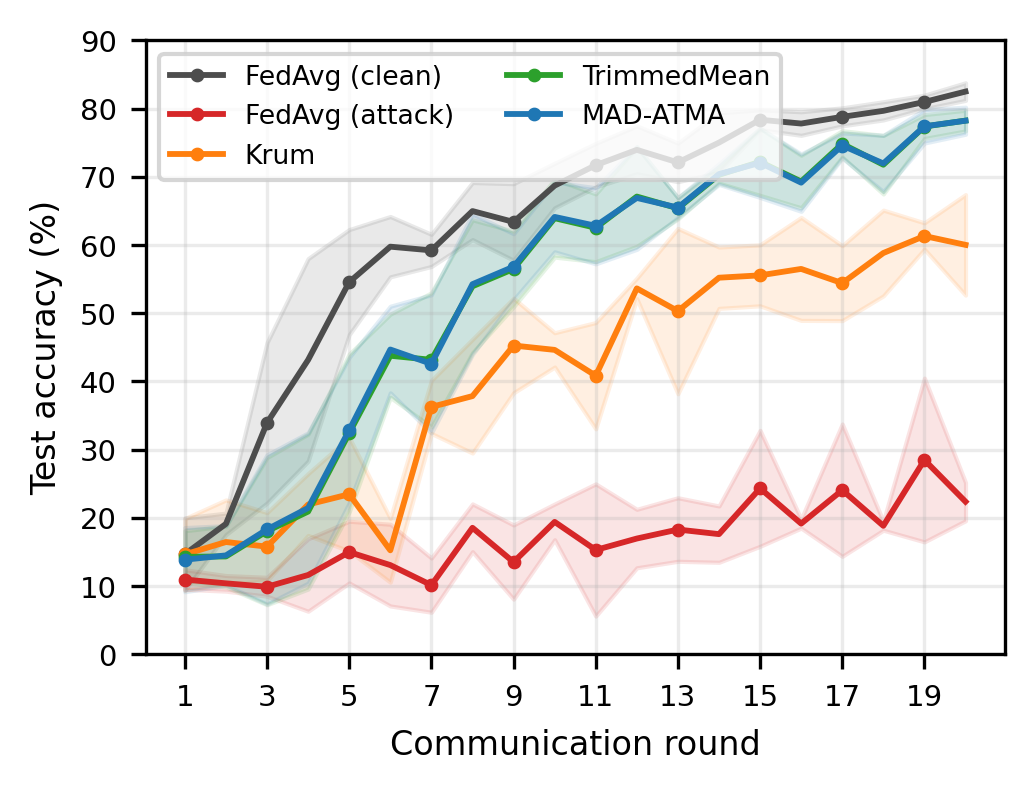
\includegraphics[width=\columnwidth]{figure1_convergence_actual.png}
\caption{Mean test accuracy across seeds 42, 43, and 44. Shaded regions show
one sample standard deviation. Every method uses the configuration in
Table~\ref{tab:configuration}.}
\label{fig:convergence}
\end{figure}

Figure~\ref{fig:convergence} shows that clean FedAvg converges fastest. Attacked
FedAvg remains unstable and low. Krum avoids malicious clients but learns more
slowly because each round retains only one client update. TrimmedMean and
MAD-ATMA combine coordinate information from several updates and finish close
to the clean baseline.

\begin{figure}[t]
\centering
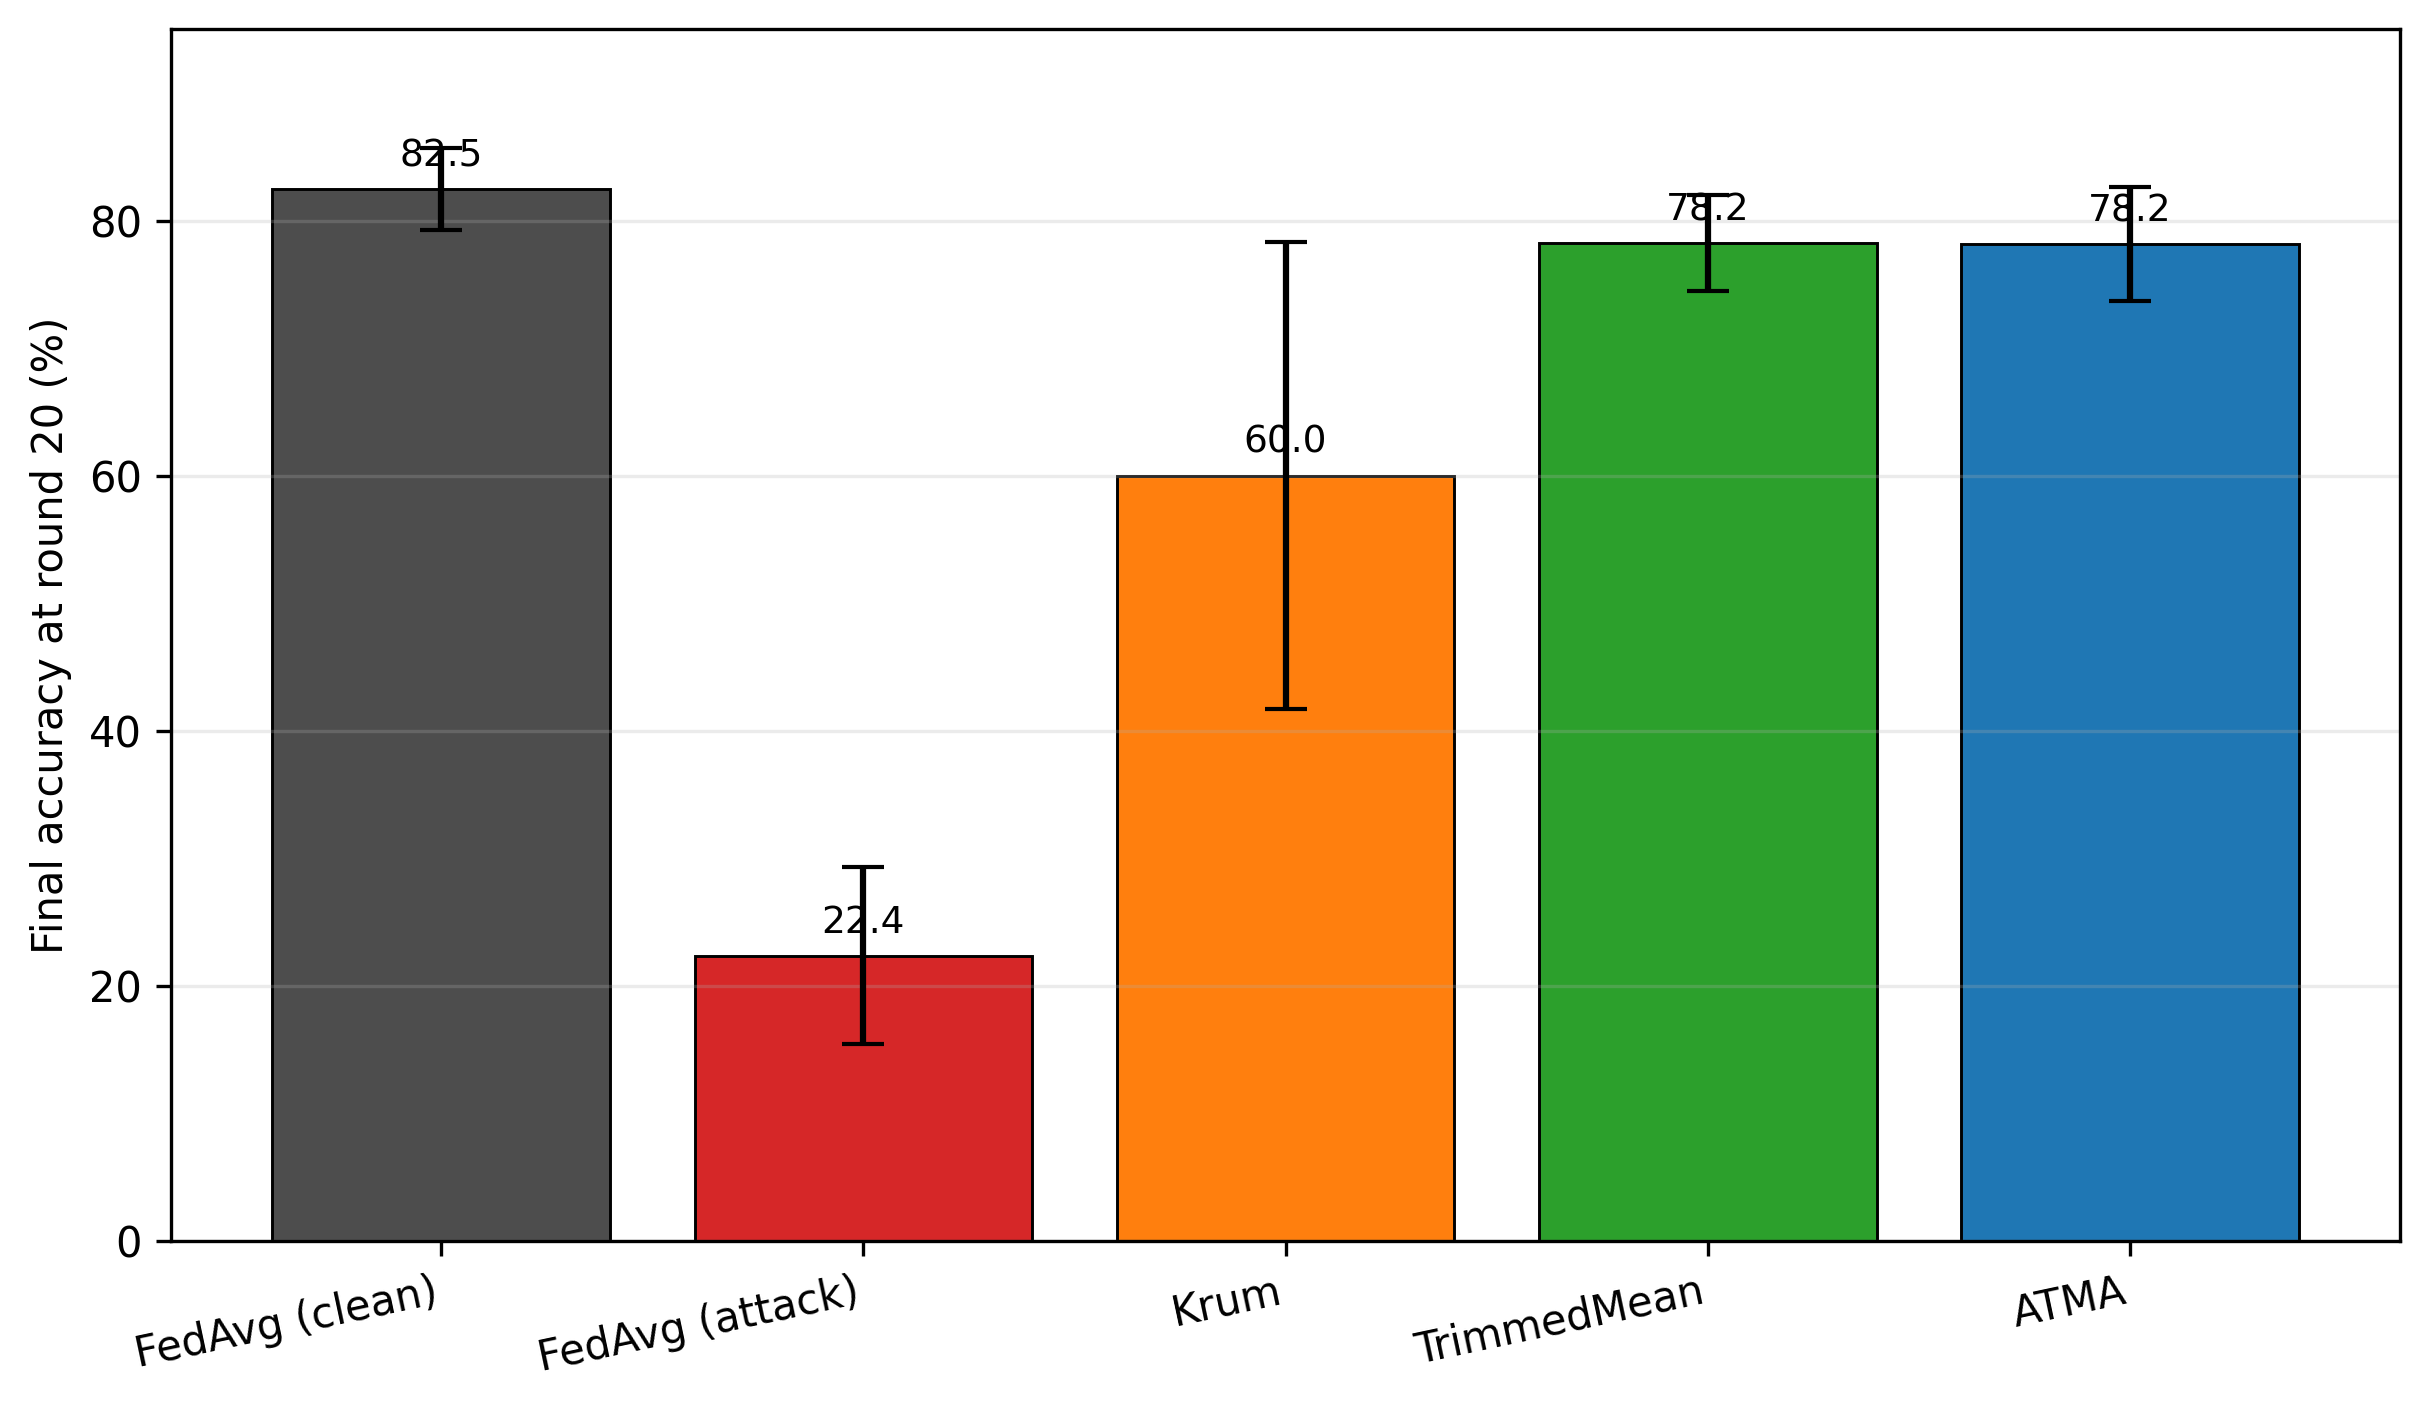
\includegraphics[width=\columnwidth]{figure2_final_accuracy_actual.png}
\caption{Final accuracy at round 20. Error bars are 95\% confidence intervals
computed with Student's $t$ distribution for three seeds.}
\label{fig:final_accuracy}
\end{figure}

MAD-ATMA and TrimmedMean differ by only $-0.01$ percentage points on average,
with $p=0.967$. Thus, no significant final-accuracy difference is detected;
this is not an equivalence test and does not prove that the methods are
identical. MAD-ATMA starts at 0.10, moves to approximately 0.15 after the first
round, and reaches final ratios of 0.213, 0.238, and 0.200 for seeds 42, 43, and
44. The observed range across all rounds is 0.150--0.238, demonstrating that
the rule is not fixed at the known 20\% Byzantine fraction.

\subsection{Detection and Krum Selection}

Across 60 MAD-ATMA rounds, there are 240 Byzantine client-round instances and
960 honest instances. MAD-ATMA produces 240 true positives, eight false
positives, no false negatives, and 952 true negatives. Precision is 96.77\%,
recall is 100\%, and F1 is 98.36\%. The number of flags per round ranges from
four to six. The eight false positives explain why the adaptive ratio sometimes
rises above 0.20. These metrics concern the explicit attack used here and
should not be interpreted as performance against the ledger-informed condition
reported below.

Corrected Krum selects an honest client in all 60 evaluated rounds. Its lower
accuracy therefore does not indicate Byzantine selection; it reflects the
utility cost of reducing a heterogeneous 20-client round to one update.

\subsection{Measured Blockchain Evidence}

\begin{table}[t]
\caption{Measured Ganache Audit Transactions}
\label{tab:blockchain_actual}
\centering
\begin{tabular}{lrr}
\toprule
Operation & Count & Mean Gas \\
\midrule
Contract deployment & 1 & 512,965 \\
Client update record & 400 & 54056 \\
Round finalization & 20 & 113991 \\
\midrule
Total measured gas & -- & 24,415,241 \\
\bottomrule
\end{tabular}
\end{table}


The audited run deploys contract \texttt{0xe78A...a8Ab}; the complete address
is preserved in the result artifact. Deployment occurs in block 1.
The run then records 400 client updates and 20 round summaries in 420
transactions, all with receipt status 1. The final block is 421. Total measured
gas including deployment is 34,647,901. All client commitments, flags, existence
bits, aggregate commitments, submitted counts, flagged counts, trim counts,
timestamps, and finalized bits pass contract read-back verification. Simulated
duplicate client and round writes revert without changing block 421. These are
local EVM execution measurements, not Ethereum-mainnet cost, latency, or
decentralization claims.

\subsection{Transparency Paradox Results}

\begin{table}[t]
\caption{Transparency Paradox Results Across Three Seeds}
\label{tab:transparency_actual}
\centering
\scriptsize
\begin{tabular}{lrrrr}
\toprule
Condition & Accuracy (\%) & Recall (\%) & Undetected (\%) & Scale \\
\midrule
Blind attacker & 78.22 $\pm$ 1.98 & 100.0 & 0.0 & 5.00 \\
Ledger-informed & 76.59 $\pm$ 1.65 & 47.5 & 52.5 & 1.63 \\
\bottomrule
\end{tabular}
\end{table}


The blind condition reproduces the main MAD-ATMA accuracies
($78.22\%\pm1.98\%$) and detects all 240 Byzantine client-round updates. The
ledger-informed condition performs 228 flag queries, implemented as 456
contract view calls including existence checks, reduces its mean attack scale
from 5.00 to 1.63, and leaves 126 of 240 Byzantine updates unflagged. Detection
recall therefore falls from 100\% to 47.5\%.

Final accuracy under ledger information is $76.59\%\pm1.65\%$, which is 1.62
percentage points below the blind condition. The seedwise reductions are 1.36,
2.01, and 1.50 points, with paired $p=0.0145$. This provides evidence of an
attacker advantage for the prespecified feedback controller: public flags improve
evasion and are associated with a small additional utility loss.

\begin{figure*}[t]
\centering
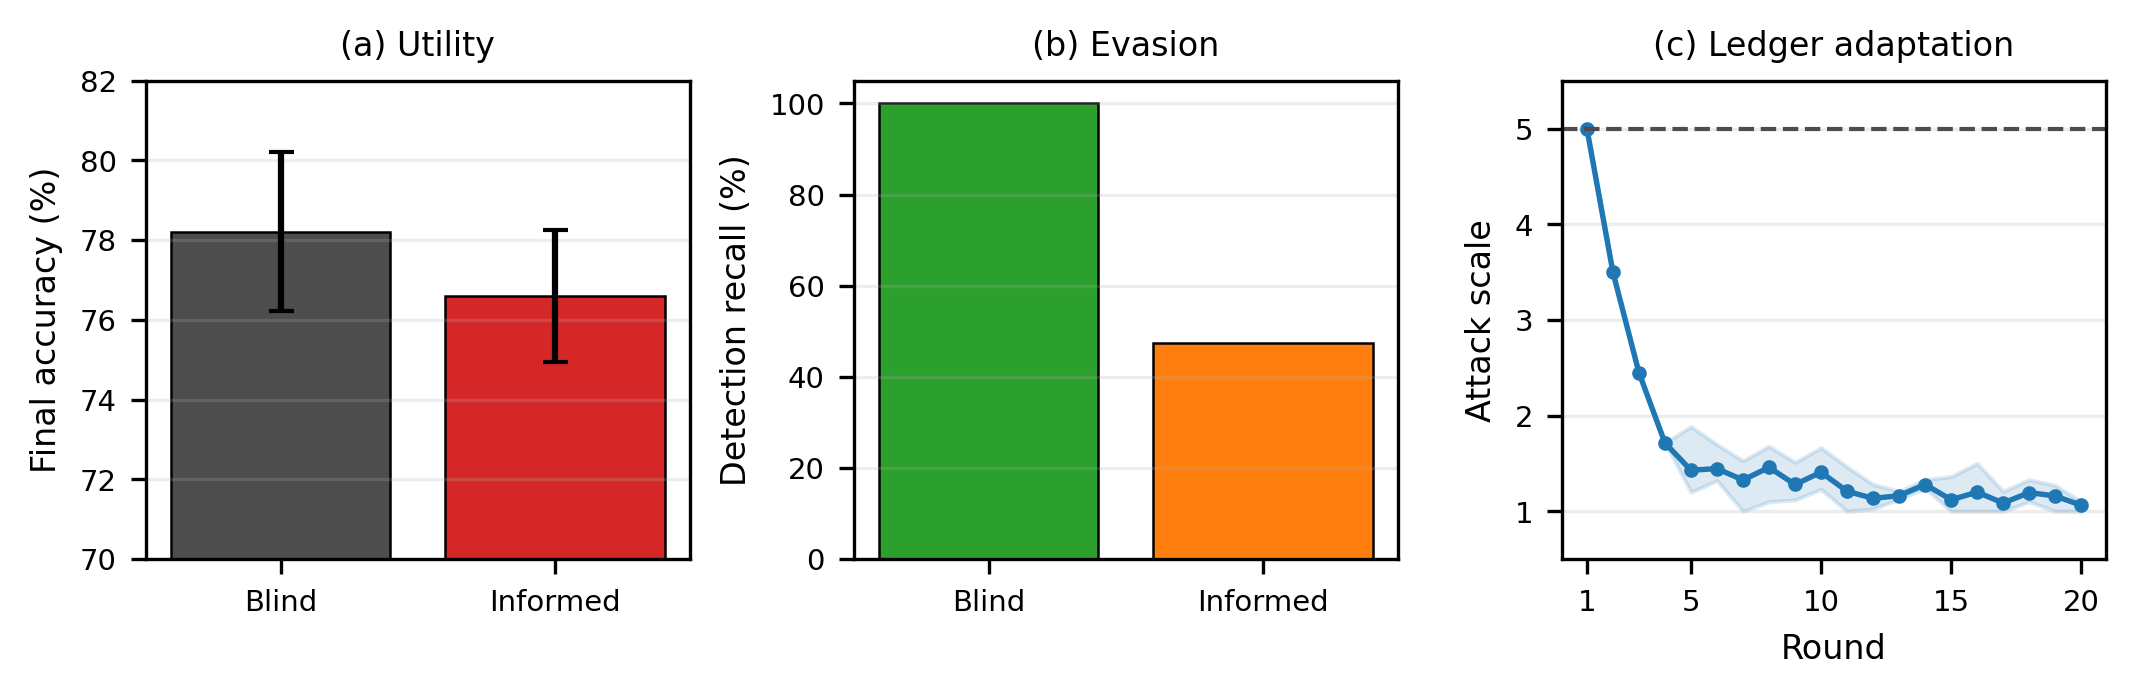
\includegraphics[width=\textwidth]{figure3_transparency_actual.png}
\caption{Measured Transparency Paradox. Blind and ledger-informed attackers use
identical training and contracts. The informed attacker reads previous-round
flags, lowers its scale, reduces detection recall, and is associated with a
1.62-point additional final-accuracy loss. The band in (c) spans the three
seeds.}
\label{fig:transparency}
\end{figure*}

The defender nevertheless retains complete committed-field audit evidence. Six
contracts record 2,400 client commitments and 120 finalized round summaries in
2,520 successful transactions; all stored client and summary fields pass
read-back verification. The 456 attacker view calls are state-free and do not
modify the ledger. Thus, the empirical resolution is a bounded tradeoff rather
than a claim that transparency is uniformly beneficial: transparency aids
adaptive evasion while preserving a complete read-back-verified record for
subsequent response.

\section{Discussion}

\subsection{Comparative Interpretation}

The comparison supports three bounded conclusions. First, the combined
label-flip and scaled-update attack severely damages both sample-weighted FedAvg
and an equal-client mean. The latter performs 9.58 points better, showing that
the reported magnitude of FedAvg degradation is partly sensitive to aggregation
weights. The experiment does not establish a monotonic causal relationship
between Byzantine sample share and accuracy. Second, coordinate-wise trimming
preserves substantially more utility than single-update Krum under the
evaluated non-IID partitions. Krum selects no Byzantine update, so its lower
accuracy is better explained by discarding information from 19 clients than by
a selection failure. Third, MAD-ATMA tracks the observed outlier fraction and
obtains essentially the same final accuracy as a static rule supplied with the
correct $f=4$ bound. Its demonstrated benefit is automatic adjustment and
diagnostic client flags, not superior accuracy.

\begin{table}[t]
\caption{Scope of Compared Robust Aggregators}
\label{tab:method_scope}
\centering
\scriptsize
\begin{tabular}{lclc}
\toprule
Method & Exact $f$? & Aggregation & Audited here?\\
\midrule
Krum & Yes & Single update & No\\
TrimmedMean & Yes & Coordinate mean & No\\
MAD-ATMA & No & Adaptive mean & Yes\\
\bottomrule
\end{tabular}
\end{table}

``No exact $f$'' in Table~\ref{tab:method_scope} does not mean parameter free.
MAD-ATMA uses a robust-score threshold, smoothing rate, and 5--25\% safety
interval. Its upper limit is intentionally different from the actual 20\%
Byzantine fraction, but future work must evaluate sensitivity to these
hyperparameters and to changing attack prevalence. FedATM of Nishimoto et
al.~\cite{nishimoto2023} also adapts trimming from model distances, but it ranks
local models and applies a distance-based retention threshold. MAD-ATMA instead
measures every update against a coordinate-median reference, standardizes those
distances with MAD, and smooths the flagged fraction into a bounded
coordinate-wise trim ratio. The later ATMA of Mukisa et
al.~\cite{mukisa2025} is variance-aware and layer-wise in an
intrusion-detection setting. These three methods therefore share adaptive
trimming terminology but use different scoring variables, threshold mechanisms,
and aggregation pipelines.

\subsection{Resolution of the Transparency Paradox}

The paradox is operationally bounded for the stated experiment by measuring both
sides of the same public information. From the attacker perspective,
previous-round flags provide useful feedback: the controller more than halves
detection recall and produces a statistically detectable 1.62-point additional
accuracy loss. From the defender perspective, this adaptation cannot erase or
rewrite the 2,520 transactions that expose submitted commitments, server flags,
trim decisions, and aggregate commitments.

These quantities are not directly commensurate, so the experiment does not
claim a universal net-benefit score. Instead, it rejects two simplistic
positions. Transparency is not attacker-neutral because it enables evasion; it
is also not equivalent to surrendering integrity because every adaptive action
still occurs against a complete committed-field write-once audit record.
Operational deployment therefore requires delayed disclosure, access control, or
detector randomization when immediate public flags create unacceptable feedback.

\subsection{Contribution of Blockchain}

The blockchain component contributes write-once commitments and reproducible
execution evidence, not robust aggregation. Detection is performed off-chain
before its output is committed. Storing SHA-256 commitments rather than
105,866-parameter tensors limits on-chain payload size. The contract prevents
the coordinator from overwriting a populated round--client slot or finalized
round, and later readers can compare local tensors and metadata with the stored
commitments.

This guarantee is narrower than saying that the complete FL system is
immutable. A trusted coordinator can still commit an incorrect hash on its
first write, and the single-node Ganache chain does not provide independent
validators. The experiments therefore validate contract execution, write-once
storage, transaction receipts, public view calls, and read-back semantics. They
do not validate
decentralized consensus, public-network latency, client authentication,
economic feasibility, or resistance to coordinator compromise.

\subsection{Limitations}

This study uses one dataset, one CNN, 20 clients, 20 rounds, three seeds, and
one combined untargeted attack. The local computation is capped at three
mini-batches per client per round. Blockchain validation uses a single-node
Ganache environment rather than independent validators. No claim is made
regarding live Layer-2 deployment, production readiness, or dollar-denominated
cost.

The primary FedAvg baseline uses canonical partition-size weighting, whereas
the robust rules are client-symmetric. The equal-client sensitivity run reduces
this comparability concern but does not replace a broader study of weighted
robust aggregators, balanced partitions, or alternative client objectives.

This study evaluates one combined untargeted attack consisting of cyclic label
flipping and scaled model updates. More sophisticated attacks, including the A
Little Is Enough attack introduced by Baruch et al.~\cite{baruch2019} and
targeted backdoor attacks studied by Sun et al.~\cite{sun2019}, remain outside
the present scope. The fixed Byzantine IDs also make detection easier to
interpret but do not test intermittent or colluding attackers. Finally, three
seeds are adequate for a reproducible correction but too few for strong claims
about population-level superiority or equivalence.

The informed attacker uses one transparent multiplicative controller and reads
only binary flags for its own four clients. It does not observe honest-client
updates, model tensors, private server state, or future decisions. Alternative
controllers, delayed disclosure, randomized detectors, different attack budgets,
and public multi-validator chains may produce a different transparency tradeoff.

\section{Conclusion}

This work empirically evaluates MAD-ATMA and provides a bounded operational
resolution of the Transparency Paradox under one reproducible protocol. A
combined label-flip and scaled-update attack reduces sample-weighted FedAvg from
82.49\% clean accuracy to 22.36\%. Krum reaches 60.01\%, while TrimmedMean and
MAD-ATMA reach 78.23\% and 78.22\%, respectively. No significant final-accuracy
difference is detected between the two trimmed methods, but MAD-ATMA adapts
without being supplied the exact $f=4$ trimming bound and provides diagnostic
client flags.

Ledger-informed adaptation reduces detection recall from 100\% to 47.5\% and is
associated with a further 1.62-point accuracy loss ($p=0.0145$), supporting the
claim that public flags can aid attacker evasion under this controller. At the
same time, six transparency contracts preserve all 2,400 client commitments and
120 round summaries, and the main audit contract preserves another 400
commitments and 20 summaries. The paradox is therefore operationally bounded as
a measured tradeoff: immediate transparency creates attacker feedback, while
write-once logging preserves evidence that the attacker cannot remove.

Future work should increase the number of seeds and rounds, test larger and
more heterogeneous datasets, evaluate partial participation, deploy the audit
contract on a multi-node or public test network, and include ALIE, model
replacement, targeted backdoor attacks, and sensitivity analysis for the MAD
threshold, trim-ratio bounds, feedback controller, and disclosure delay.

\section*{Declarations}

\subsection*{Declaration of Competing Interests}

The authors declare that they have no known competing financial interests or
personal relationships that could have appeared to influence the work reported
in this article.

\subsection*{Acknowledgment}

The authors would like to thank the Electrical Engineering Department, Faculty
of Engineering, Universitas Brawijaya, and the Laboratory of Internet of Things
and Human Centered Design, Faculty of Vocational Studies, Universitas Brawijaya,
for providing computational resources and supercomputer support for this
research.

\subsection*{Data Availability}

The experiment script, robust aggregation module, Solidity source, raw JSON
results, generated tables, and figure-generation code are packaged with this
revision. MNIST is publicly available from its original source and through
\texttt{torchvision}. The exact R4 code and results, including the equal-client
sensitivity and Transparency Paradox artifacts, are supplied in the
supplementary archive
\path{18579_R4_REPRODUCIBILITY_SUPPLEMENT.zip}. A public project repository is
identified in \cite{repository2026}; the supplementary archive remains the
authoritative artifact for this R4 journal review.

\subsection*{AI Use and Declaration of Generative AI Use}

During the preparation of this revision, the authors used OpenAI Codex to assist
with code inspection and editing, experiment orchestration, consistency checks,
language editing, and LaTeX/Word document preparation. Experiments were executed
locally from author-reviewed scripts, and figures were generated
programmatically from recorded JSON results. After using this tool, the authors
reviewed and edited the code, outputs, figures, and text as needed and take full
responsibility for the content of the publication.

\small
\begin{thebibliography}{20}

\bibitem{mcmahan2017}
H. B. McMahan, E. Moore, D. Ramage, S. Hampson, and B. Ag\"uera y Arcas,
``Communication-efficient learning of deep networks from decentralized data,''
in \emph{Proc. 20th Int. Conf. Artif. Intell. Statist. (AISTATS)}, vol. 54,
2017, pp. 1273--1282.

\bibitem{kairouz2021}
P. Kairouz, H. B. McMahan, B. Avent, \emph{et al.},
``Advances and open problems in federated learning,''
\emph{Found. Trends Mach. Learn.}, vol. 14, no. 1--2, pp. 1--210, 2021,
doi: 10.1561/2200000083.

\bibitem{mothukuri2021}
V. Mothukuri, R. M. Parizi, S. Pouriyeh, Y. Huang, A. Dehghantanha, and
G. Srivastava, ``A survey on security and privacy of federated learning,''
\emph{Future Gener. Comput. Syst.}, vol. 115, pp. 619--640, Feb. 2021,
doi: 10.1016/j.future.2020.10.007.

\bibitem{tariq2024}
A. Tariq, M. A. Serhani, F. M. Sallabi, E. S. Barka, T. Qayyum, H. M. Khater,
and K. A. Shuaib, ``Trustworthy federated learning: A comprehensive review,
architecture, key challenges, and future research prospects,''
\emph{IEEE Open J. Commun. Soc.}, vol. 5, pp. 4920--4998, 2024,
doi: 10.1109/OJCOMS.2024.3438264.

\bibitem{hu2024}
K. Hu, S. Gong, Q. Zhang, C. Seng, M. Xia, and S. Jiang,
``An overview of implementing security and privacy in federated learning,''
\emph{Artif. Intell. Rev.}, vol. 57, art. no. 204, Jul. 2024,
doi: 10.1007/s10462-024-10846-8.

\bibitem{feng2025}
Y. Feng, Y. Guo, Y. Hou, \emph{et al.}, ``A survey of security threats in
federated learning,'' \emph{Complex Intell. Syst.}, vol. 11, art. no. 165,
Jan. 2025, doi: 10.1007/s40747-024-01664-0.

\bibitem{blanchard2017}
P. Blanchard, E. M. El Mhamdi, R. Guerraoui, and J. Stainer,
``Machine learning with adversaries: Byzantine tolerant gradient descent,''
in \emph{Advances in Neural Information Processing Systems}, vol. 30, 2017.

\bibitem{yin2018}
D. Yin, Y. Chen, R. Kannan, and P. Bartlett,
``Byzantine-robust distributed learning: Towards optimal statistical rates,''
in \emph{Proc. 35th Int. Conf. Mach. Learn. (ICML)}, vol. 80, 2018,
pp. 5650--5659.

\bibitem{zhao2022}
L. Zhao, J. Jiang, B. Feng, Q. Wang, C. Shen, and Q. Li,
``SEAR: Secure and efficient aggregation for Byzantine-robust federated
learning,'' \emph{IEEE Trans. Dependable Secure Comput.}, vol. 19, no. 5,
pp. 3329--3342, Sep./Oct. 2022, doi: 10.1109/TDSC.2021.3093711.

\bibitem{baruch2019}
M. Baruch, G. Baruch, and Y. Goldberg,
``A little is enough: Circumventing defenses for distributed learning,''
in \emph{Advances in Neural Information Processing Systems}, vol. 32, 2019.

\bibitem{sun2019}
Z. Sun, P. Kairouz, A. T. Suresh, and H. B. McMahan,
``Can you really backdoor federated learning?''
arXiv:1911.07963, 2019.

\bibitem{kim2020}
H. Kim, J. Park, M. Bennis, and S.-L. Kim,
``Blockchained on-device federated learning,''
\emph{IEEE Commun. Lett.}, vol. 24, no. 6, pp. 1279--1283, Jun. 2020,
doi: 10.1109/LCOMM.2019.2921755.

\bibitem{lu2020}
Y. Lu, X. Huang, K. Zhang, S. Maharjan, and Y. Zhang,
``Blockchain empowered asynchronous federated learning for secure data sharing
in Internet of Vehicles,''
\emph{IEEE Trans. Veh. Technol.}, vol. 69, no. 4, pp. 4298--4311, Apr. 2020,
doi: 10.1109/TVT.2020.2973651.

\bibitem{zhu2023}
J. Zhu, J. Cao, D. Saxena, S. Jiang, and H. Ferradi,
``Blockchain-empowered federated learning: Challenges, solutions, and future
directions,'' \emph{ACM Comput. Surv.}, vol. 55, no. 11, art. no. 240,
pp. 1--31, Feb. 2023, doi: 10.1145/3570953.

\bibitem{hallaji2024}
E. Hallaji, R. Razavi-Far, M. Saif, B. Wang, and Q. Yang,
``Decentralized federated learning: A survey on security and privacy,''
\emph{IEEE Trans. Big Data}, vol. 10, no. 2, pp. 194--213, Apr. 2024,
doi: 10.1109/TBDATA.2024.3362191.

\bibitem{zhang2024}
Y. Zhang, D. Zeng, J. Luo, X. Fu, G. Chen, Z. Xu, and I. King,
``A survey of trustworthy federated learning: Issues, solutions, and
challenges,'' \emph{ACM Trans. Intell. Syst. Technol.}, vol. 15, no. 6,
art. no. 112, pp. 1--47, 2024, doi: 10.1145/3678181.

\bibitem{nishimoto2023}
K. Nishimoto, Y.-H. Chiang, H. Lin, and Y. Ji,
``FedATM: Adaptive trimmed mean based federated learning against model poisoning
attacks,'' in \emph{Proc. IEEE 97th Veh. Technol. Conf. (VTC2023-Spring)},
Florence, Italy, Jun. 2023, pp. 1--5,
doi: 10.1109/VTC2023-Spring57618.2023.10200010.

\bibitem{mukisa2025}
K. J. Mukisa, L. A. C. Ahakonye, D.-S. Kim, and J.-M. Lee,
``Blockchain-augmented FL IDS for non-IID edge-IoT data using adaptive trimmed
mean aggregation,''
\emph{IEEE Internet Things J.}, vol. 12, no. 21, pp. 45150--45159, Nov. 2025,
doi: 10.1109/JIOT.2025.3598832.

\bibitem{lecun1998}
Y. LeCun, L. Bottou, Y. Bengio, and P. Haffner,
``Gradient-based learning applied to document recognition,''
\emph{Proc. IEEE}, vol. 86, no. 11, pp. 2278--2324, Nov. 1998,
doi: 10.1109/5.726791.

\bibitem{repository2026}
R. A. Atmoko, ``Byzantine-robust federated learning with blockchain:
Reproducibility repository,'' 2026. [Online]. Available:
\url{https://github.com/vokasitibrawijaya/byzantine-robust-fl-blockchain}.
Accessed: Jun. 25, 2026.

\end{thebibliography}

\end{document}
